\section{Alloy}
\lstset{
  language=alloy,
  basicstyle=\small\ttfamily,
  breaklines=true,
  showstringspaces=false
}
\lstinputlisting{4Alloy/res/second_model.als}

\subsection{Generated World}
\begin{figure}[h]
  \centering
  %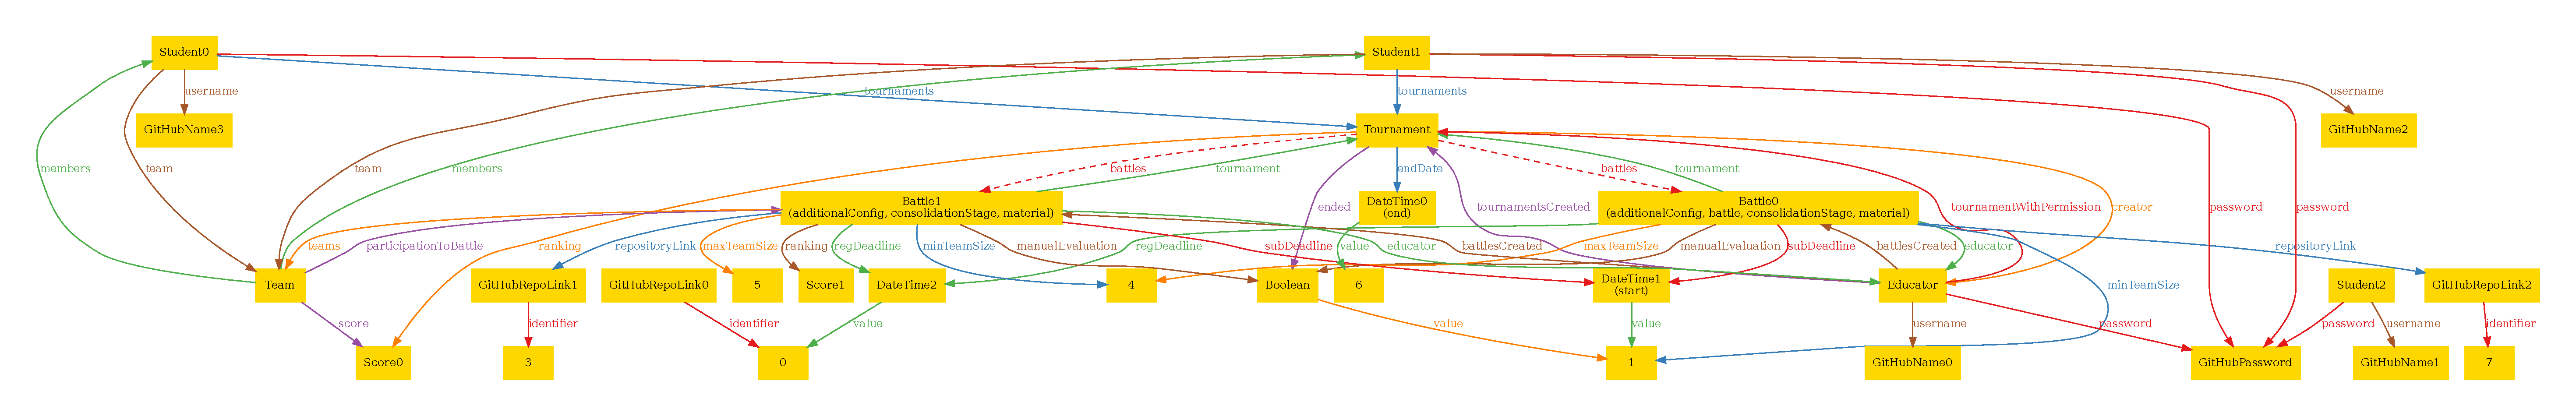
\includegraphics[width=1\linewidth]{RASD/4Alloy/res/general.pdf}
  \caption{The world generated by running \textit{general} projected over nine signatures (ABS, Boolean, CodeTest, DateTime, GitHubName, Int, Macrovariables, Password, SourceCode) in order to be more comprehensible}
\end{figure}

\begin{figure}[h]
  \centering
  %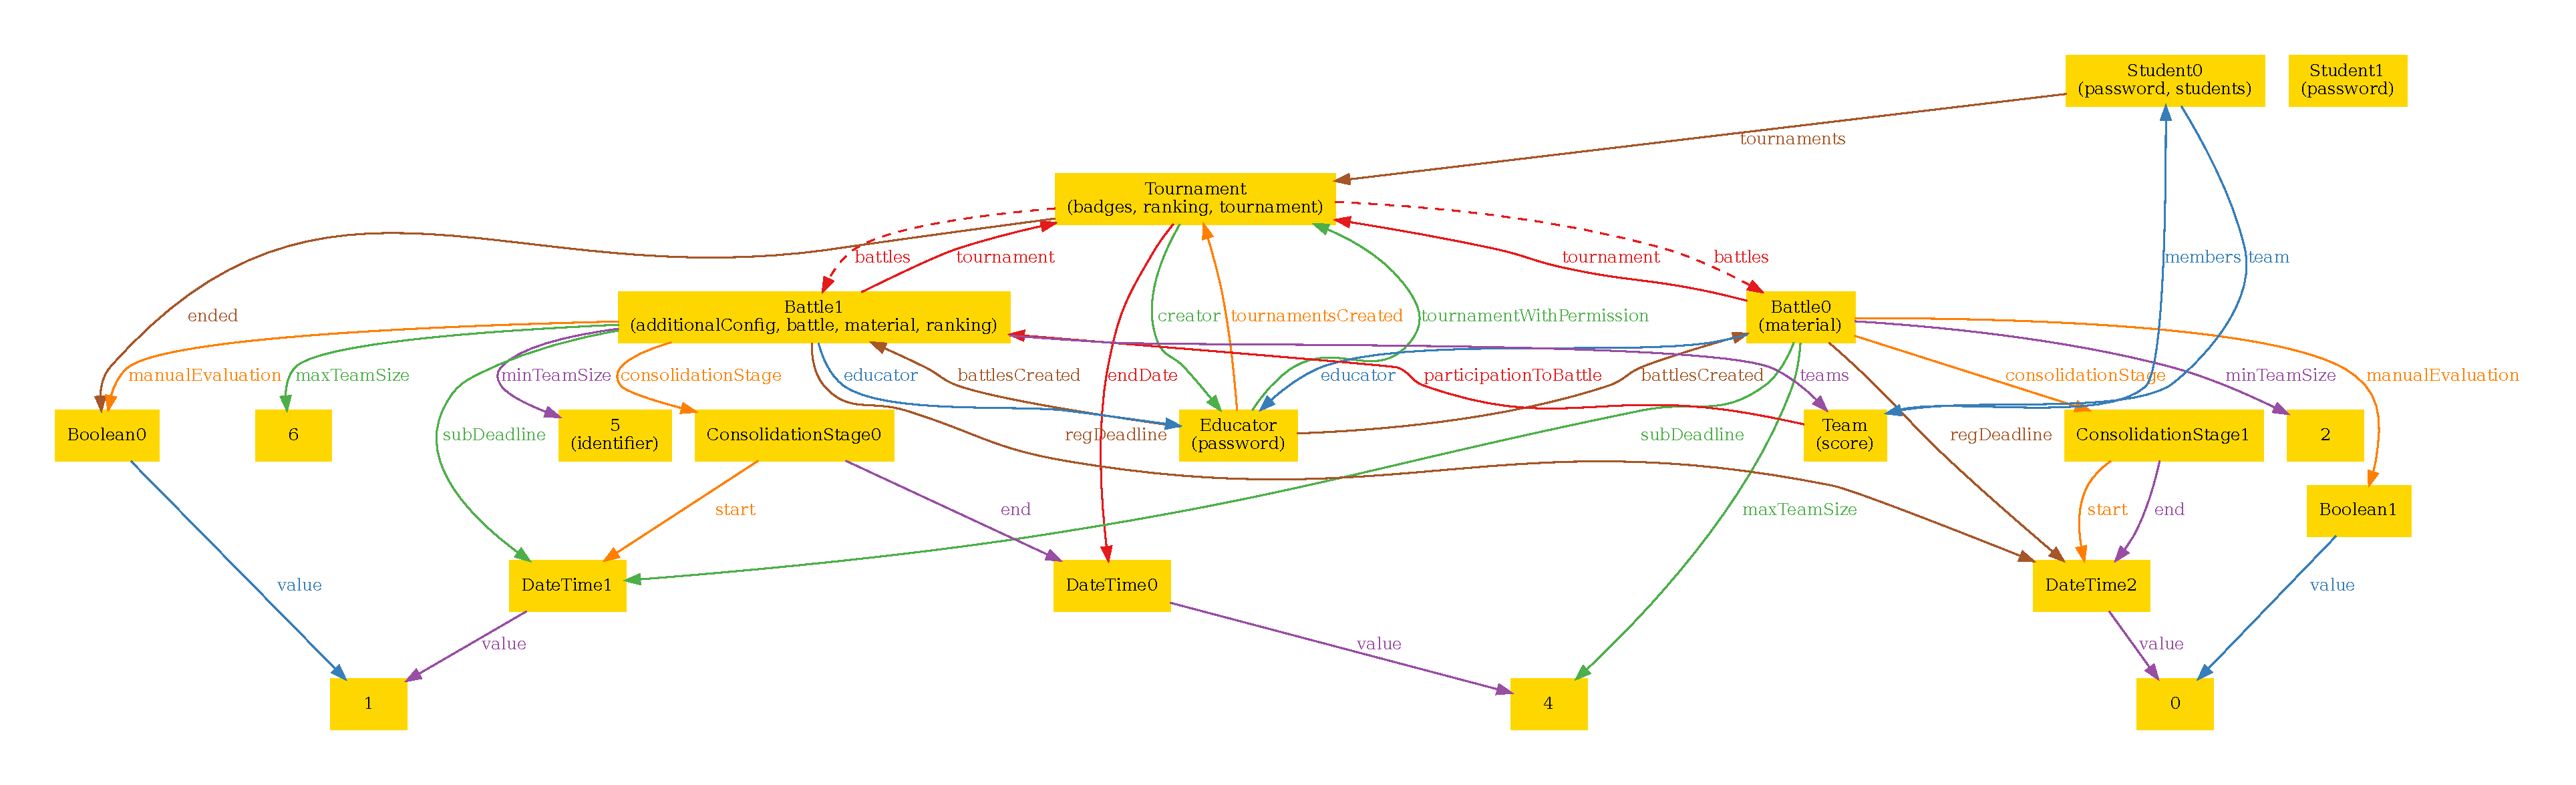
\includegraphics[width=1\linewidth]{RASD/4Alloy/res/noManualEvaluation.pdf}
  \caption{The world generated by running \textit{noManualEvaluation} projected over nine signatures (ABS, Boolean, CodeTest, DateTime, GitHubName, Int, Macrovariables, Password, SourceCode) in order to be more comprehensible. This world exploit the situation where there is no manual evaluation for one battle out of two. It is useful in order to see the right aim of the model}
\end{figure}

The representation of the world at the instant 1 is here omitted due to the fact it only modifies one of the value among the signatures.